%% ============ PARTE A ============
\section{El algoritmo: puentes con Tarjan (Parte A)}

\subsection{¿Qué es un puente y para qué sirve?}
Sea $G=(V,E)$ un grafo no dirigido. Una arista $e\in E$ es un \textbf{puente} si al quitarla aumenta
el número de componentes conexas de $G$. Dicho de otra forma, es una conexión que no tiene ``plan B'':
no existe otro camino entre sus extremos.

Puentes es un \textbf{algoritmo}, no una estructura de datos, así que no representa un TDA. Sirve para
encontrar los puntos únicos de falla de una red: el cable cuya caída deja equipos aislados, la carretera
que si se cierra deja incomunicado un pueblo, o la línea de una red eléctrica que no tiene respaldo.
También es el primer paso para otros algoritmos, por ejemplo para hallar las componentes
2-arista-conexas (lo que queda al quitar todos los puentes).

\subsection{Cómo funciona}
El algoritmo de Tarjan hace \textbf{un solo DFS} y guarda dos números por nodo:
\begin{itemize}
  \item $\mathit{tin}[v]$: el momento en que el DFS descubre a $v$ (un contador que sube en 1 cada vez).
  \item $\mathit{low}[v]$: el menor $\mathit{tin}$ al que se puede llegar desde el subárbol de $v$ bajando
        por aristas de árbol y usando \emph{a lo más una} back edge al final.
\end{itemize}
Al entrar a $u$ se hace $\mathit{tin}[u]=\mathit{low}[u]=\text{timer}$. Luego se recorre su lista de
adyacencia:
\begin{itemize}
  \item Si el vecino $v$ ya fue visitado (y no es la arista por la que llegamos), es una back edge:
        $\mathit{low}[u]=\min(\mathit{low}[u],\mathit{tin}[v])$.
  \item Si no fue visitado, es una arista de árbol: se llama a $\mathrm{dfs}(v)$ y al volver
        $\mathit{low}[u]=\min(\mathit{low}[u],\mathit{low}[v])$.
\end{itemize}
\noindent\textbf{Criterio:} la arista de árbol $(u,v)$ es puente si y solo si
\[ \mathit{low}[v] > \mathit{tin}[u]. \]

Dos detalles de implementación que hacen falta para que funcione en todos los casos:
\begin{enumerate}
  \item La arista padre se salta \textbf{por id de arista}, no por vértice padre. Si se saltara por
        vértice, con dos aristas paralelas entre $u$ y $v$ la segunda también se ignoraría y la primera
        saldría mal como puente.
  \item El DFS se lanza desde \textbf{cada nodo no visitado}, para que funcione en grafos desconectados.
\end{enumerate}

\subsection{¿Por qué es correcto?}
En un DFS de un grafo no dirigido solo hay dos tipos de aristas: de árbol y back edges (que unen un nodo
con un ancestro suyo); no hay aristas cruzadas. Tomemos una arista de árbol $(u,v)$:
\begin{itemize}
  \item Si $\mathit{low}[v]\le\mathit{tin}[u]$, hay un nodo del subárbol de $v$ con una back edge hacia $u$
        o hacia un ancestro de $u$. Esa back edge forma un ciclo que contiene a $(u,v)$, así que al quitar
        $(u,v)$ sigue habiendo camino: no es puente.
  \item Si $\mathit{low}[v]>\mathit{tin}[u]$, ninguna arista sale del subárbol de $v$ hacia $u$ o más
        arriba. Como no hay aristas cruzadas, la única conexión entre el subárbol de $v$ y el resto es
        $(u,v)$: al quitarla el subárbol queda aislado, entonces es puente.
\end{itemize}
Además, una back edge nunca es puente, porque siempre está dentro de un ciclo (ella más el camino de
árbol entre sus extremos). Por eso basta revisar las aristas de árbol.

\subsection{Estructuras que usa por dentro}
\begin{itemize}
  \item \textbf{Grafo con listas de adyacencia}: \texttt{vector<vector<Arista>>}, donde cada
        \texttt{Arista} guarda el vecino \texttt{to} y el \texttt{id} de la arista (necesario para las
        aristas paralelas). Ocupa $O(V+E)$.
  \item \textbf{Arreglos} \texttt{tin}, \texttt{low} de tamaño $V$ (empiezan en $-1$ = no visitado) y
        \texttt{esPuente} de tamaño $E$.
  \item \textbf{Pila de recursión} del DFS, que en el peor caso (un camino) llega a profundidad $V$.
        En la animación se dibuja a la derecha como ``pila de recursión''.
\end{itemize}

\subsection{Ejemplo animado}
La escena \texttt{Demo} usa \texttt{graphs/demo.txt} (8 nodos, 9 aristas): un cuadrado $0$-$1$-$2$-$3$,
un triángulo $4$-$5$-$6$, la arista $2$-$4$ entre ambos y la arista $6$-$7$. La animación reproduce la
traza real que imprime \texttt{bin/tarjan}. Los valores finales son:

\begin{center}
\begin{tabular}{lcccccccc}
\toprule
nodo & 0 & 1 & 2 & 3 & 4 & 5 & 6 & 7\\
\midrule
$\mathit{tin}$ & 0 & 1 & 2 & 3 & 4 & 5 & 6 & 7\\
$\mathit{low}$ & 0 & 0 & 0 & 0 & 4 & 4 & 4 & 7\\
\bottomrule
\end{tabular}
\end{center}

La back edge $3$-$0$ hace que $\mathit{low}=0$ suba por $3,2,1$, así que el cuadrado no tiene puentes.
En cambio, $\mathit{low}[4]=4>\mathit{tin}[2]=2$ y $\mathit{low}[7]=7>\mathit{tin}[6]=6$, por lo que los
puentes son $e_4=(2,4)$ y $e_8=(6,7)$. Se necesitaron 26 operaciones instrumentadas ($8$ nodos
descubiertos $+ 2\cdot 9 = 18$ entradas de adyacencia revisadas), justo $V+2E$.

\begin{center}
\IfFileExists{captura_intro.png}{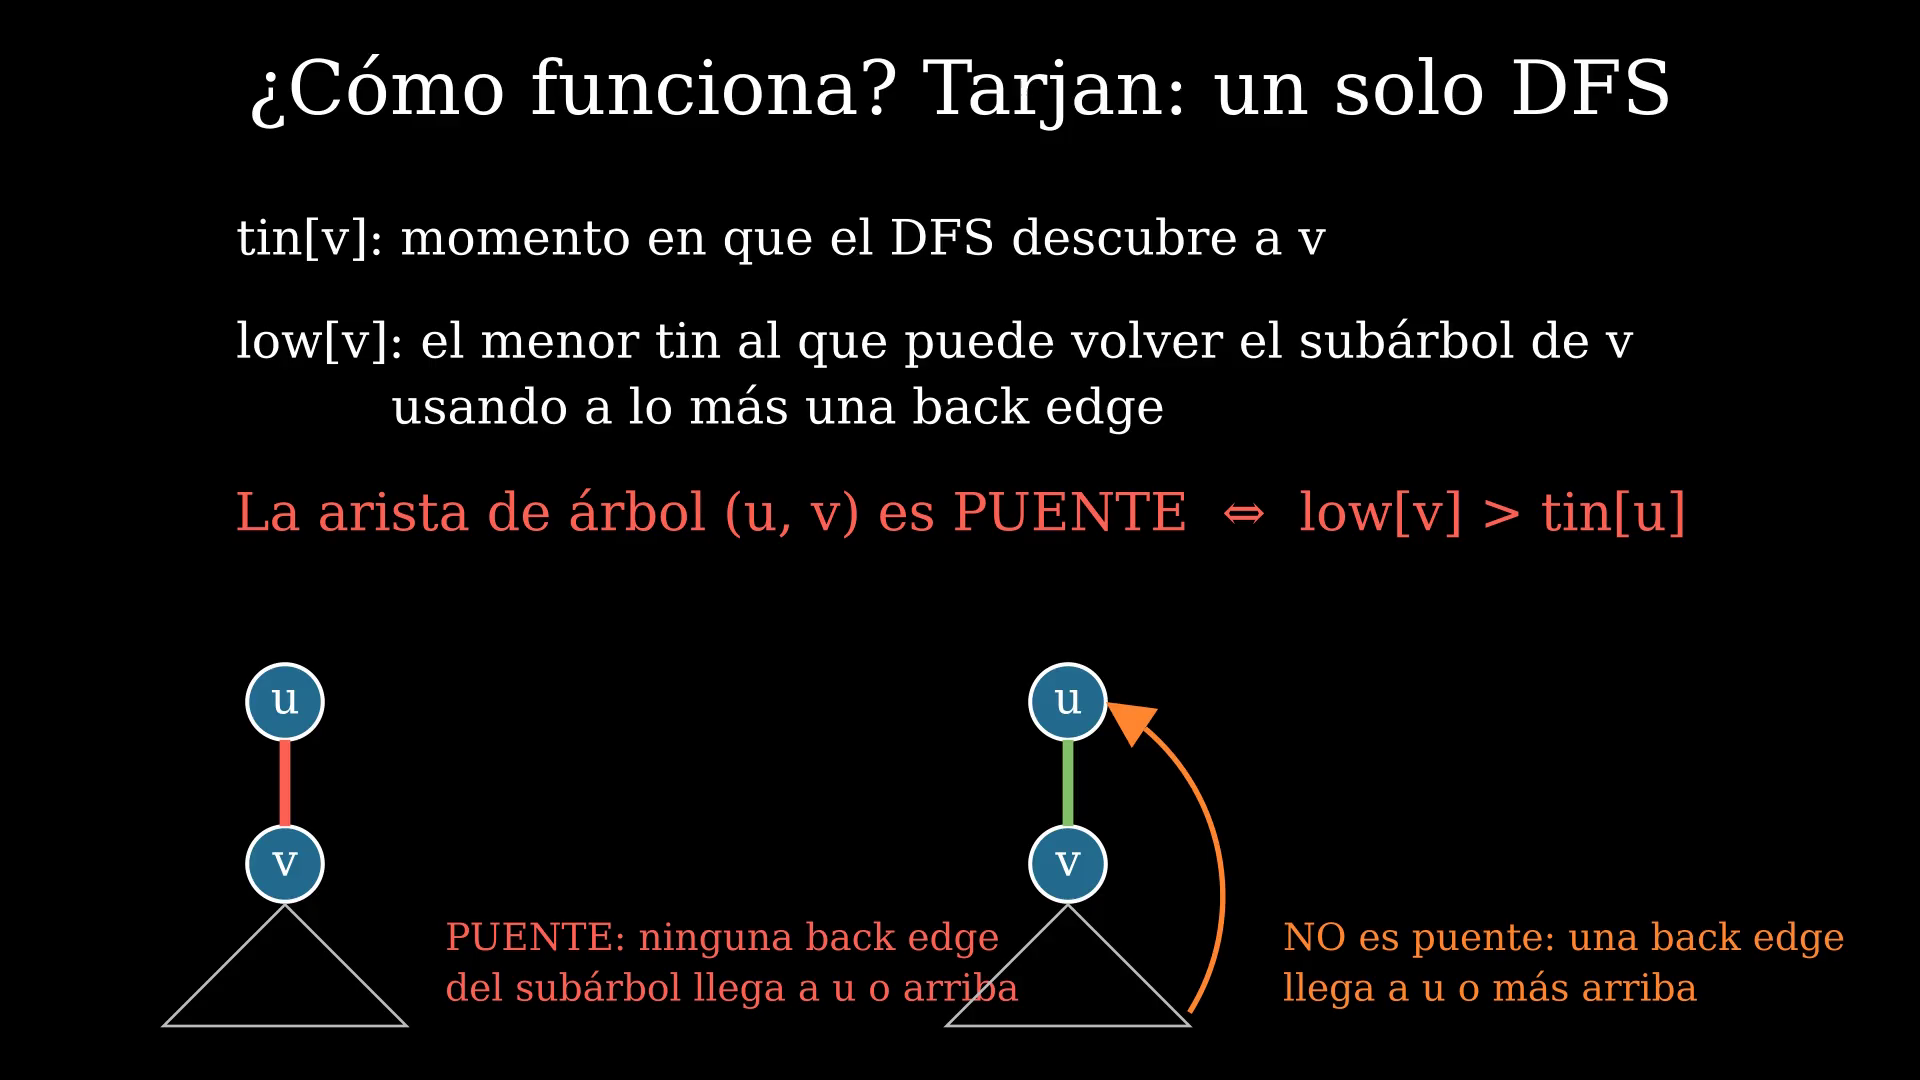
\includegraphics[width=0.48\textwidth]{captura_intro.png}}{}\hfill
\IfFileExists{captura_demo.png}{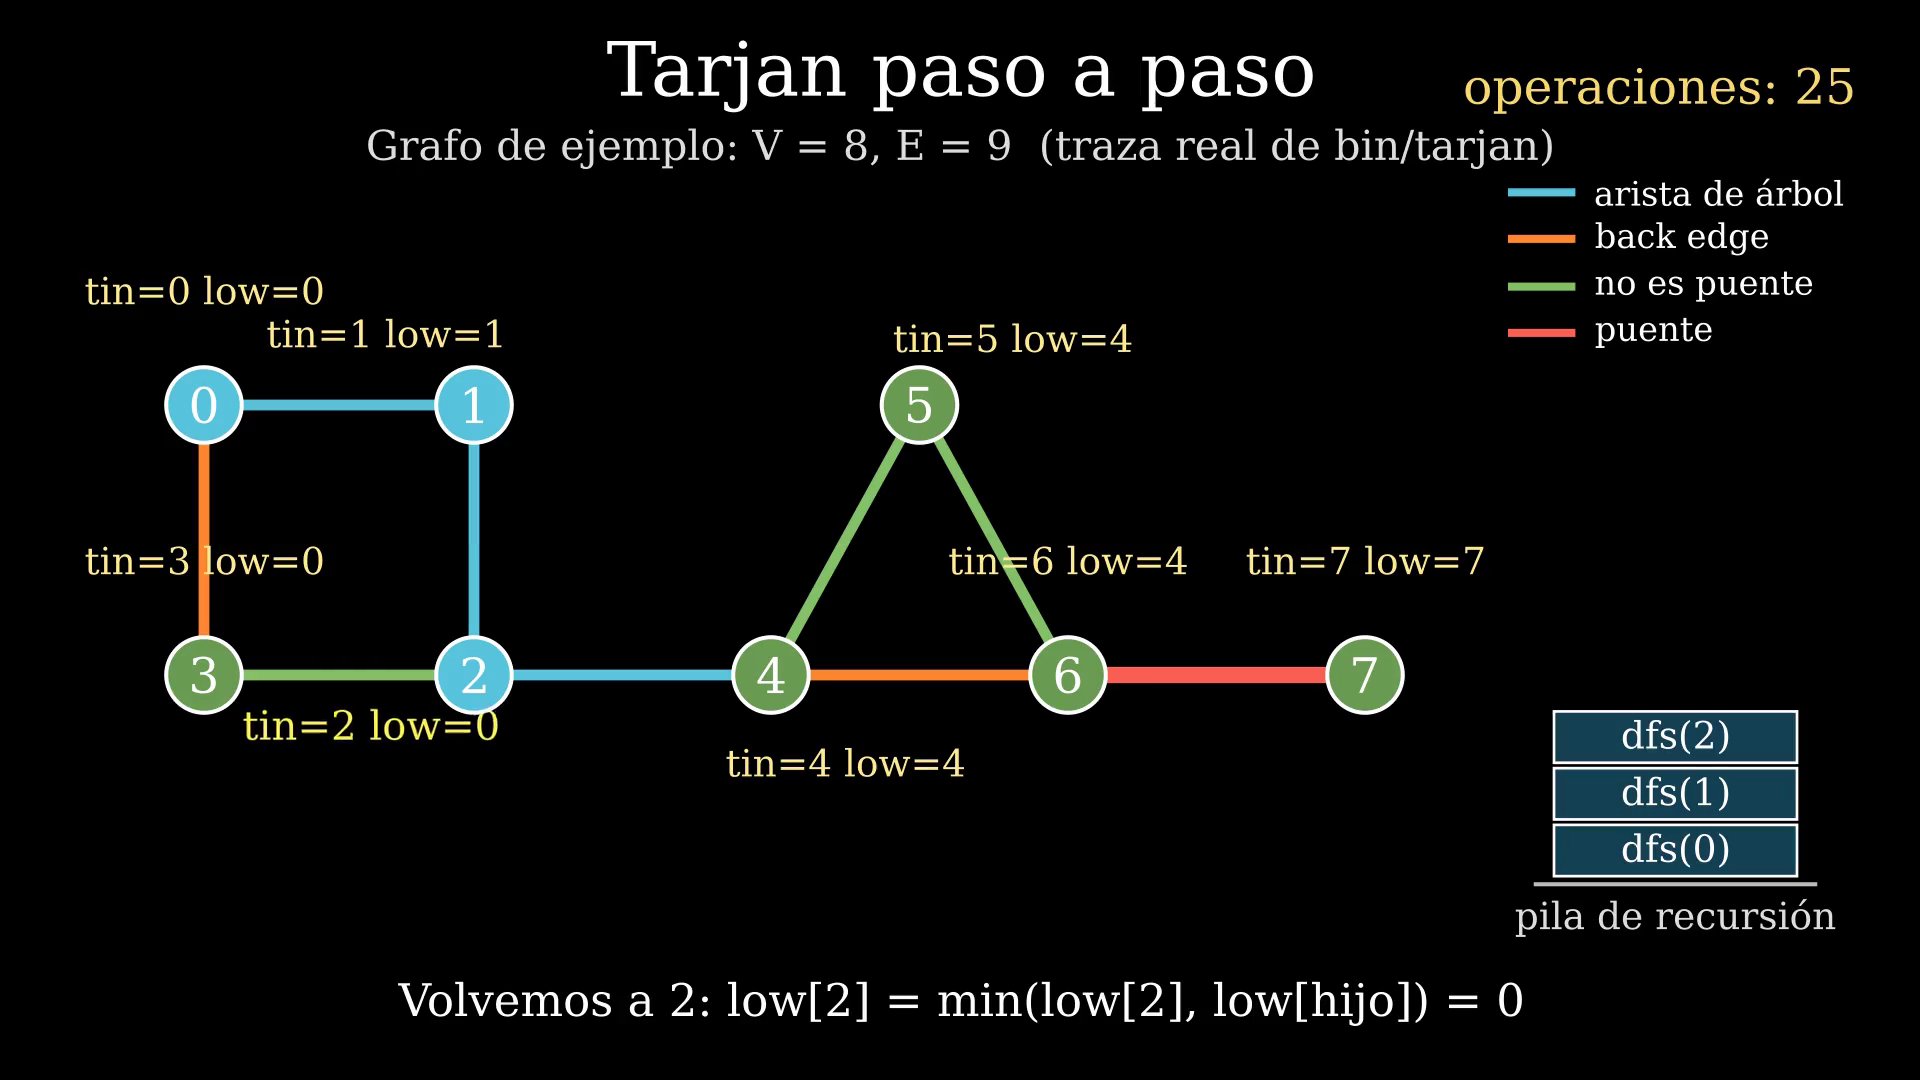
\includegraphics[width=0.48\textwidth]{captura_demo.png}}{}\\
{\small Izquierda: criterio del puente en la escena \texttt{Intro}. Derecha: escena \texttt{Demo} a mitad
de la ejecución, con \texttt{tin}/\texttt{low} y la pila de recursión.}
\end{center}

\subsection{Escenas de la Parte A}
El video de la Parte A (\texttt{video\_parteA.mp4}, unos 2 minutos) une la portada con estas tres escenas
mediante \texttt{sh scripts/join\_A.sh}.
\begin{itemize}
  \item \texttt{manim/intro\_A.py} (\texttt{Intro}): qué es un puente con el ejemplo de dos ciudades
        unidas por una carretera, para qué sirve y la idea de $\mathit{tin}$/$\mathit{low}$. Cuál arista
        es puente no está puesto a mano: la escena corre \texttt{bin/tarjan --compact} sobre
        \texttt{graphs/intro.txt}.
  \item \texttt{manim/codigo\_A.py} (\texttt{Codigo}): muestra la función \texttt{dfs} leída directamente de
        \texttt{src/tarjan.cpp} (sin las líneas de la traza) y resalta paso a paso las líneas clave: inicializar
        $\mathit{tin}/\mathit{low}$, saltar la arista padre por id, back edge, recursión, actualizar $\mathit{low}$
        y el criterio del puente.
  \item \texttt{manim/demo\_A.py} (\texttt{Demo}): ejecución paso a paso sobre \texttt{graphs/demo.txt},
        reutilizando \texttt{TarjanPlayer} de \texttt{common.py} y agregando la pila de recursión.
        Al final se quitan los puentes y se colorean los bloques que quedan.
\end{itemize}
La implementación \texttt{src/tarjan.cpp} pasa \texttt{scripts/cross\_check.py}: coincide con la fuerza
bruta en 500 grafos aleatorios (con aristas paralelas, autolazos y nodos aislados) y produce exactamente
la misma traza que la versión de referencia en todos los grafos de \texttt{graphs/}.
